%% 
%% Copyright 2007, 2008, 2009 Elsevier Ltd
%% 
%% This file is part of the 'Elsarticle Bundle'.
%% ---------------------------------------------
%% 
%% It may be distributed under the conditions of the LaTeX Project Public
%% License, either version 1.2 of this license or (at your option) any
%% later version.  The latest version of this license is in
%%    http://www.latex-project.org/lppl.txt
%% and version 1.2 or later is part of all distributions of LaTeX
%% version 1999/12/01 or later.
%% 
%% The list of all files belonging to the 'Elsarticle Bundle' is
%% given in the file `manifest.txt'.
%% 

%% Template article for Elsevier's document class `elsarticle'
%% with numbered style bibliographic references
%% SP 2008/03/01

\documentclass[preprint,1p]{elsarticle}
\biboptions{numbers,sort&compress}

%% Use the option review to obtain double line spacing
%% \documentclass[authoryear,preprint,review,12pt]{elsarticle}

%% Use the options 1p,twocolumn; 3p; 3p,twocolumn; 5p; or 5p,twocolumn
%% for a journal layout:
%% \documentclass[final,1p,times]{elsarticle}
%% \documentclass[final,1p,times,twocolumn]{elsarticle}
%% \documentclass[final,3p,times]{elsarticle}
%% \documentclass[final,3p,times,twocolumn]{elsarticle}
%% \documentclass[final,5p,times]{elsarticle}
%% \documentclass[final,5p,times,twocolumn]{elsarticle}

%% For including figures, graphicx.sty has been loaded in
%% elsarticle.cls. If you prefer to use the old commands
%% please give \usepackage{epsfig}

%% The amssymb package provides various useful mathematical symbols
\usepackage{amssymb}
\usepackage{lineno}
\usepackage{hyperref}
\usepackage{siunitx}
\usepackage{multirow}
\usepackage{wasysym}
%\usepackage[percent]{overpic}
%\usepackage[usenames,dvipsnames,svgnames,table]{xcolor}
%\usepackage{cleveref}

%% The amsthm package provides extended theorem environments
%% \usepackage{amsthm}

%% The lineno packages adds line numbers. Start line numbering with
%% \begin{linenumbers}, end it with \end{linenumbers}. Or switch it on
%% for the whole article with \linenumbers.
%% \usepackage{lineno}

\journal{Nucl. Instrum. Meth. A}

\begin{document}

\linenumbers

\begin{frontmatter}

%% Title, authors and addresses

%% use the tnoteref command within \title for footnotes;
%% use the tnotetext command for theassociated footnote;
%% use the fnref command within \author or \address for footnotes;
%% use the fntext command for theassociated footnote;
%% use the corref command within \author for corresponding author footnotes;
%% use the cortext command for theassociated footnote;
%% use the ead command for the email address,
%% and the form \ead[url] for the home page:
%% \title{Title\tnoteref{label1}}
%% \tnotetext[label1]{}
%% \author{Name\corref{cor1}\fnref{label2}}
%% \ead{email address}
%% \ead[url]{home page}
%% \fntext[label2]{}
%% \cortext[cor1]{}
%% \address{Address\fnref{label3}}
%% \fntext[label3]{}

\title{Studies of uniformity of 50~$\mu$m low-gain avalanche detectors
at the Fermilab test beam.}

%% use optional labels to link authors explicitly to addresses:
%% \author[label1,label2]{}
%% \address[label1]{}
%% \address[label2]{}

\author[1]{A.~Apresyan\corref{cor}}\ead{apresyan@fnal.gov}
\author[2]{S.~Xie}
\author[2]{C.~Pena}
\author[5,7]{R.~Arcidiacono}
\author[5]{N.~Cartiglia}
\author[8]{M.~Carulla}
\author[1]{G.~Derylo}
\author[5]{M.~Ferrero}
\author[8]{D.~Flores}
\author[4]{P.~Freeman}
\author[4]{Z.~Galloway}
\author[9]{A.~Ghassemi}
\author[3]{H.~Al Ghoul}
\author[1]{L.~Gray}
\author[8]{S.~Hidalgo}
\author[9]{S.~Kamada}
\author[1]{S.~Los}
\author[5]{M.~Mandurrino}
\author[8]{A.~Merlos}
\author[3]{N.~Minafra}
\author[1]{A.~Ronzhin}
\author[8]{G.~Pellegrini}
\author[8]{D.~Quirion}
\author[3]{C.~Royon}
\author[4]{H.~Sadrozinski}
\author[4]{A.~Seiden}
\author[5]{V.~Sola}
\author[2]{M.~Spiropulu}
\author[5]{A.~Staiano}
\author[1]{L.~Uplegger}
\author[9]{K.~Yamamoto}
\author[9]{K.~Yamamura}

\address[1]{Fermi National Accelerator Laboratory, Batavia, IL, USA}
\address[2]{California Institute of Technology, Pasadena, CA, USA}
\address[3]{University of Kansas, KS, USA}
\address[4]{SCIPP, University of California Santa Cruz, CA, USA}
\address[5]{INFN, Torino, Italy}
\address[6]{Universit\`a di Torino, Torino, Italy}
\address[7]{Universit\`a del Piemonte Orientale, Italy}
\address[8]{Centro Nacional de Microelectr\'{o}nica (IMB-CNM-CSIC), Barcelona, Spain}
\address[9]{Hamamatsu Photonics (HPK), Hamamatsu, Japan}
\cortext[cor]{Corresponding author}

\begin{abstract}
%% Text of abstract
In this paper we report measurements of the uniformity of time resolution, signal
amplitude, and charged particle detection efficiency across the sensor surface
of low-gain avalanche detectors (LGAD). Comparisons of the performance of sensors
with different doping concentrations and different active thicknesses are
presented, as well as their temperature dependance and radiation tolerance up to
$6\times 10^{14}$~n/cm$^2$. Results were obtained at the Fermilab test beam
facility using 120 GeV proton beams, and a high precision pixel tracking
detector. LGAD sensors manufactured by the Centro Nacional de Microelectr\'{o}nica (CNM) and
Hamamatsu Photonics (HPK) were studied. The uniformity of the
sensor response in pulse height before irradiation was found to have a
2\% spread. The signal detection efficiency and timing resolution in the sensitive areas before irradiation
were found to be 100\%  and 30-40~\si{ps}, respectively. A ``no-response'' area between pads was
measured to be about 130~$\mu$m for CNM and 170$\mu$m for HPK sensors. After a
neutron fluence of $6\times 10^{14}$~n/cm$^2$ the CNM sensor exhibits a large
gain variation of up to a factor of $2.5$ when comparing metalized and non-metalized
sensor areas. An irradiated CNM sensor achieved a time resolution of 30~ps for the
metalized area and 40~ps for the non-metalized area, while 
a HPK sensor irradiated to the same fluence achieved a 30~\si{ps} time resolution.
\end{abstract}

\begin{keyword}
%% keywords here, in the form: keyword \sep keyword

%% PACS codes here, in the form: \PACS code \sep code
Silicon \sep Timing \sep LGAD \sep Test Beam
%% MSC codes here, in the form: \MSC code \sep code
%% or \MSC[2008] code \sep code (2000 is the default)

\end{keyword}

\end{frontmatter}

\tableofcontents

%% \linenumbers

%% main text
\section{Introduction} 

Future colliders, including the high luminosity upgrade of the Large Hadron
Collider (HL-LHC) at CERN, will operate with an order of magnitude higher
instantaneous luminosity compared to what has been achieved at the
large hadron collider (LHC) so far.
With the increased instantaneous luminosity, the rate of simultaneous
interactions per bunch crossing (pileup) is projected to reach an average of 140
to 200. The large amount of pileup increases the difficulties in separating 
particles from the hard scattering interaction with those
produced in different pileup interactions. In particular, the ability to discriminate between
jets produced in the events of interests, especially those associated with vector 
boson fusion processes, and jets produced by pileup interactions will be
degraded. Additionally, the efficiency to identify high $p_{\mathrm{T}}$ isolated electrons
and muons will be severely reduced due to the high density of pileup particles
in their vicinity. The missing transverse energy resolution will also deteriorate, and several
other physics objects performance metrics will also suffer the
detrimental effects of pileup.


One way to mitigate the pileup effects mentioned above, complementary to
precision tracking methods, is to perform a time of arrival measurement
associated with each particle. Such a measurement with a precision of about
30-40~\si{ps}, will reduce the effective amount of pileup by a factor of 10,
given that the spread in collision time of the pileup interactions at HL-LHC is
foreseen to be approximately 200~\si{ps}. It has been previously shown that a
precision of better than $20$~\si{ps} can be achieved for electromagnetic
showers measured with silicon sampling
calorimeters~\cite{Apresyan201662,Apresyan2017_NSSMIC,AKCHURIN201731} using
traditional planar silicon detectors. In this paper, we report results of
particle beam measurements with thin low-gain avalanche detectors (LGAD) that
have been shown to achieve time resolutions around
30~\si{ps}~\cite{Cartiglia201783, PELLEGRINI201412}. LGAD are envisioned to be
used in the CMS and ATLAS experiment upgrades for HL-LHC in order to overcome
the event reconstruction challenges posed by the high rate of concurrent
collisions per beam crossing. The implemented regions of pseudorapidity ($\eta$)
are: $|\eta|>1.5$, and $2.4 < |\eta| < 4.2 $ for CMS and ATLAS, respectively. In
order to achieve the desired timing precision across a large area of the
detectors, the sensors will need to provide high uniformity of signal response
and timing resolution. In this paper, we perform detailed measurements of the
performance of LGAD sensors produced by Centro Nacional de Microelectr\'{o}nica
(CNM) and Hamamatsu Photonics (HPK) exposed to the 120~GeV proton beam at
Fermilab. Utilizing high-precision tracking detectors we extract position
dependence of the charged-particle detection efficiency, signal pulse height,
signal timestamp, and time resolution of 50~$\mu$m LGAD sensors. We also compare
the uniformity of 50 and 80~$\mu$m LGAD sensors. Uniformity and and time
resolution of the HPK and CNM sensors irradiated to an equivalent neutron
fluence of $6\times 10^{14}$~n/cm$^2$ are also presented. Detailed measurements
of irradiated HPK sensors were presented in Ref.~\cite{Galloway:2017gfx}.

The paper is organized as follows: the experimental setup is described in
Sec.~\ref{sec:setup}; the tested LGAD sensors and their operating conditions are
listed in Sec.~\ref{sec:sensors}; readout electronics used in the measurements
are described in Sec.~\ref{sec:boards}; algorithms used in the event
reconstruction are described in Sec.~\ref{sec:timestampReco}; beam test results
are presented in Sec.~\ref{sec:results}, followed by the conclusion in
Sec.~\ref{sec:conclusion}.

\section{Experimental Setup} 
\label{sec:setup}

%We performed the test-beam measurements at the Fermilab Test-beam
%Facility%

Test-beam measurements were performed at the Fermilab Test-beam Facility (FTBF)
which provided a $120$~GeV proton beam from the Fermilab Main Injector
accelerator. The Devices Under Test (DUTs) were mounted on a remotely operated
motorized stage, placed inside the pixel telescope detector~\cite{KWAN2016162}.
The latter provides better than 10~$\mu$m position resolution for charged
particles impinging on the DUT. Additionally, a Photek~240 micro-channel plate
(MCP-PMT) detector~\cite{Anderson:2015gha, MCPFastCaloNIMA,
Ronzhin2015288,Ronzhin201552} was placed furthest downstream, and provided a
very precise reference timestamp. Its precision has been previously
measured to be less than $7$~ps~\cite{Ronzhin2015288}. A schematic diagram and
photograph of the experimental area are shown in Fig.~\ref{fig:DragonBoxDiagram}
and Fig.~\ref{fig:DragonBox}, respectively. 

The DAQ system for the DUTs and the Photek MCP-PMT is based on a CAEN V1742
digitizer board~\cite{CAENDRS}, which provides digitized waveforms sampled at 5
GS/s, and with one ADC count corresponding to 0.25~mV. The CAEN digitizer was
voltage- and time-calibrated using the procedure described in
Ref.~\cite{Kim201467}. One of the main parameters of DAQ system for precise time
measurements is the ``electronic time resolution'', defined as the measured time
jitter between two signals that are split from the same source. These two
signals are used as ``start'' and ``stop'' signals to electronic system
measuring the time interval between them. The electronic time resolution of the
CAEN V1742 digitizer was measured to be less than 4~ps, and thus, its impact on
the timing measurements presented in these studies can be neglected. The DAQ for
the pixel telescope is based on the CAPTAN system developed at
Fermilab~\cite{KWAN2016162}. The track-reconstruction is performed using the
Monicelli software package developed specifically for the test-beam application. 

\begin{figure}[htbp] 
\centering
\includegraphics[width=0.75\textwidth]{figs/BeamSetup.pdf} 
\caption{A schematic diagram of the test-beam setup is shown. The $t_0$ and $t_1$ are defined in Section 4.} 
\label{fig:DragonBoxDiagram} 
\end{figure} 

The DUTs were placed inside the telescope box described in
Ref.\cite{KWAN2016162}, and mounted on an aluminum mechanical support structure.
The telescope box can be moved remotely in both the horizontal and vertical
directions in order to align the DUTs with the beam. The aluminum support
structure for the DUTs provide both mechanical stability and are
equipped with Peltier cooling elements that were used in this study to operate
the DUTs at $-10^{\circ}$ and $-20^{\circ}$~C.

\begin{figure}[htbp] 
\centering
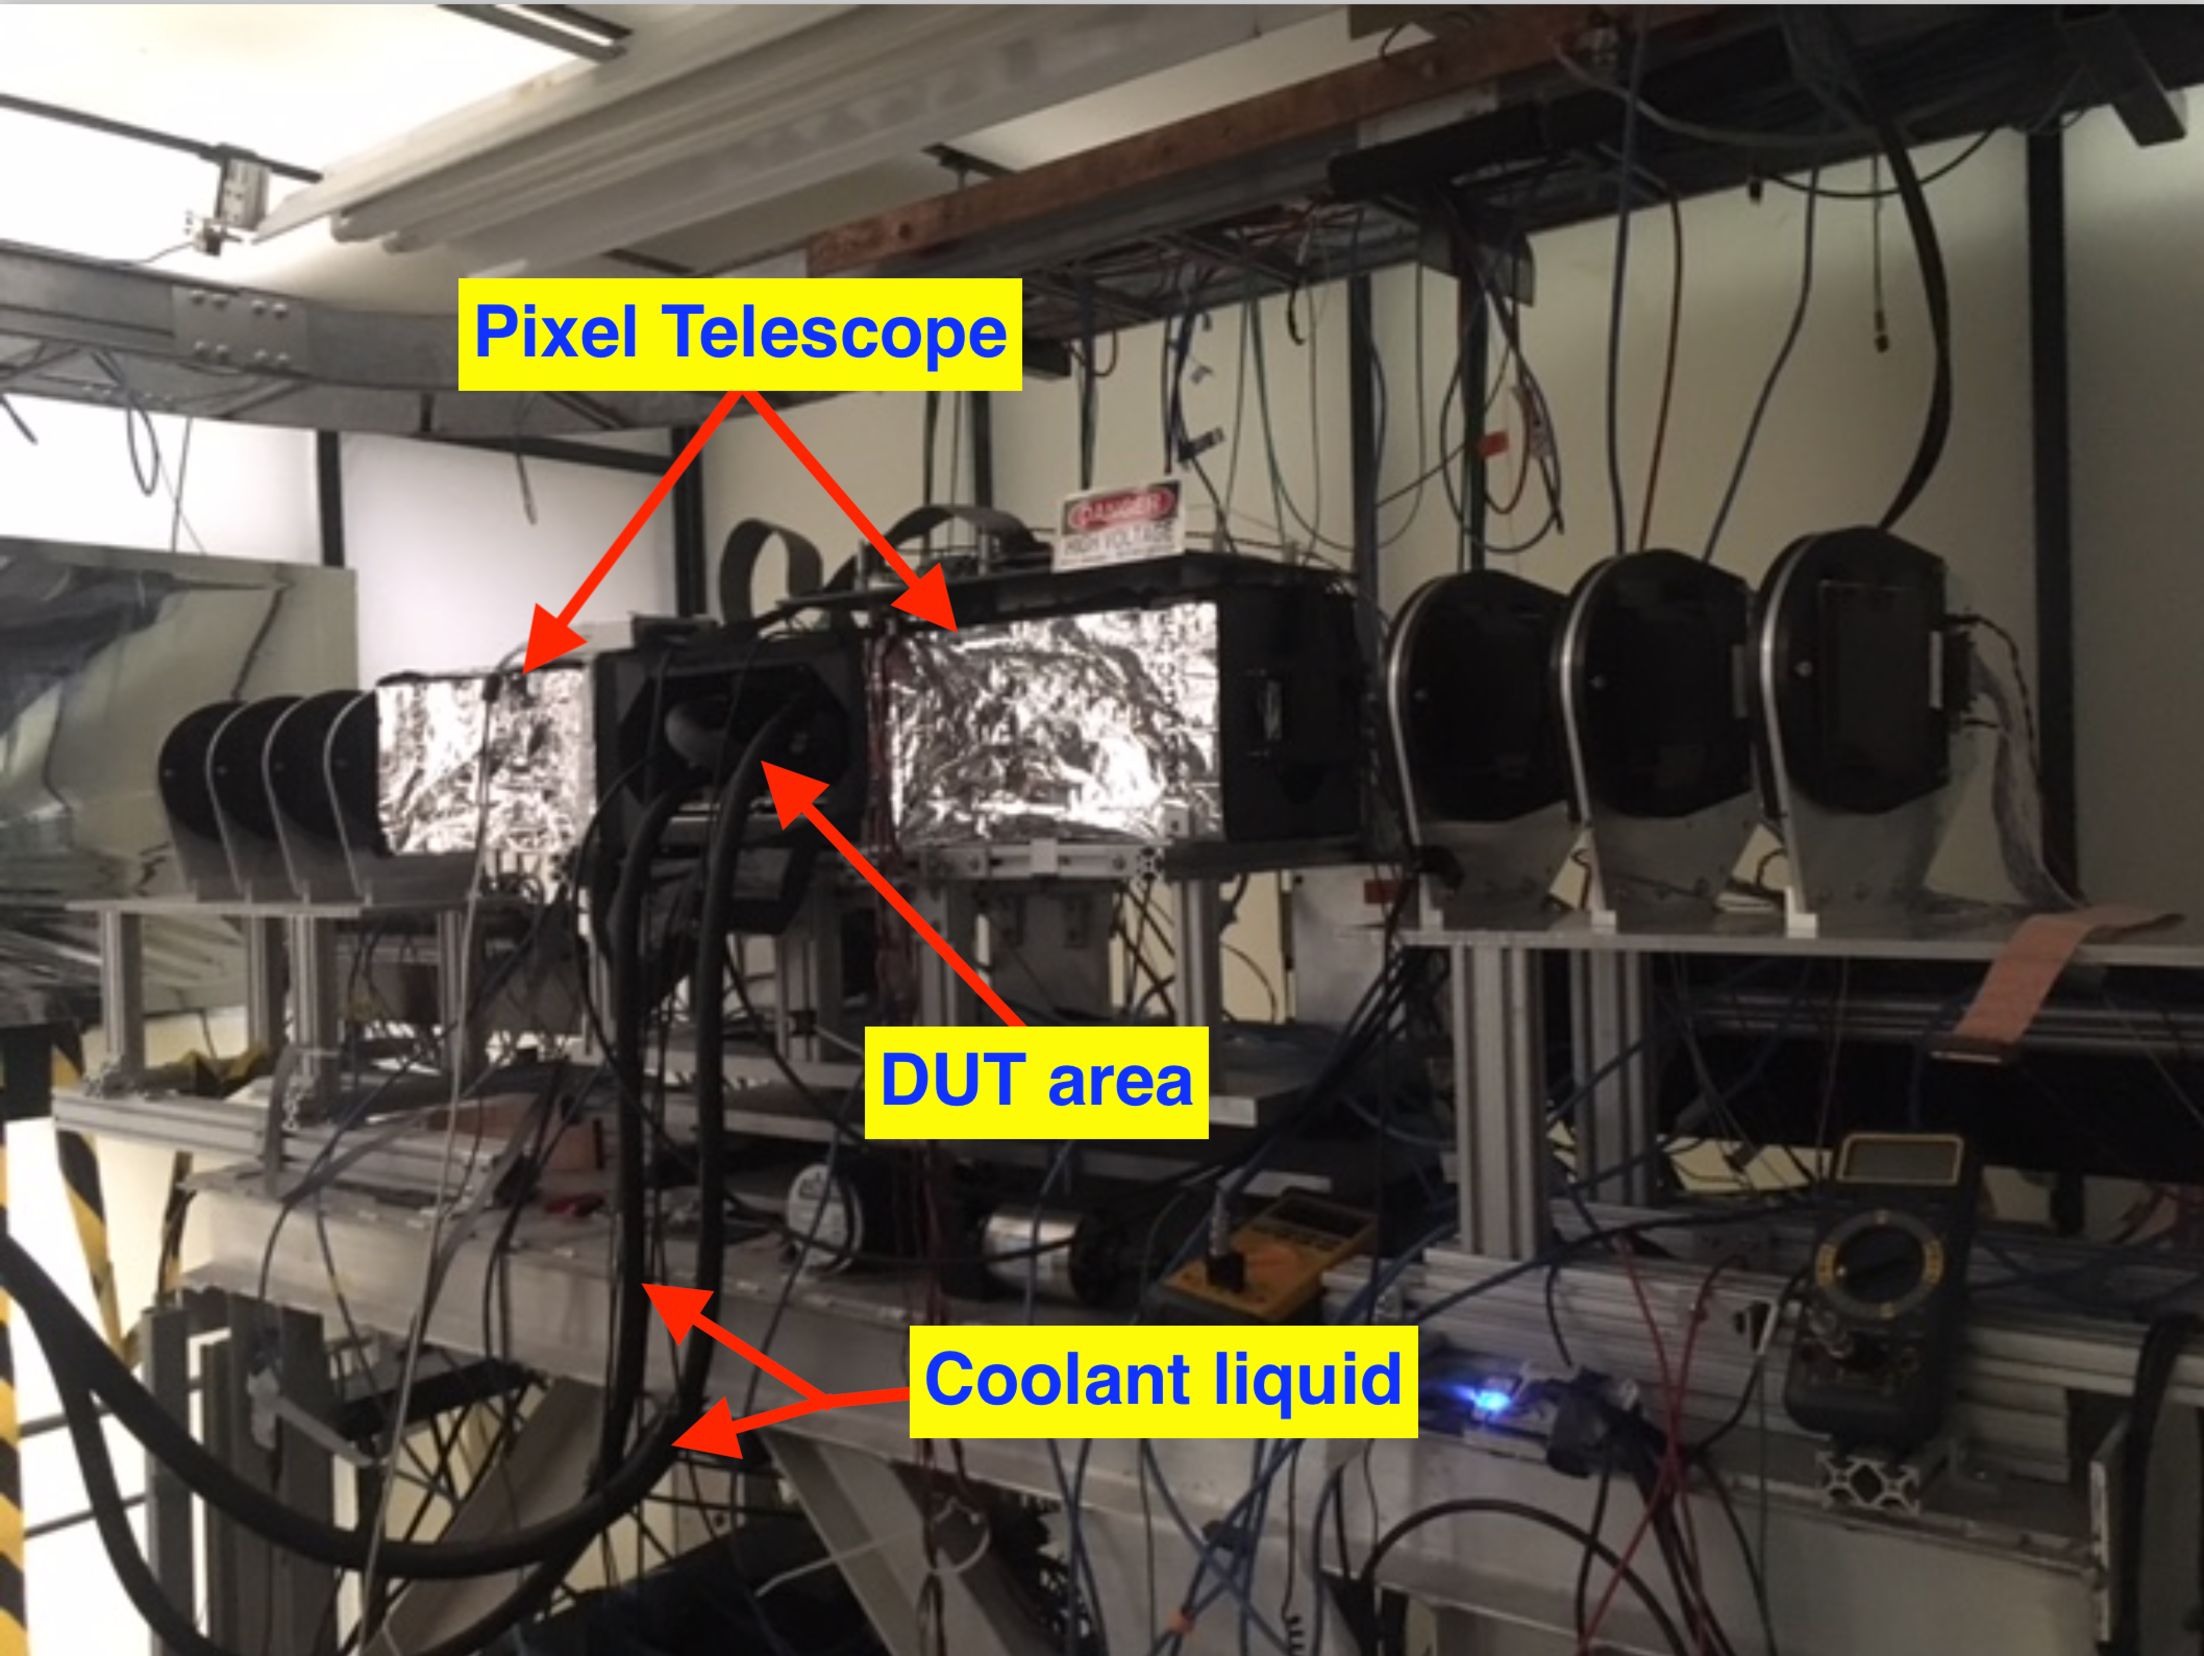
\includegraphics[width=0.75\textwidth]{figs/TB_dragonBox.pdf} 
\caption{A picture of the experimental area. Thea pixel telescope detectors are placed inside the 
electrostatic-discharge shielded boxes on the two sides of the DUT area. Cooling liquid for 
the Peltier elements inside the DUT area is provided by the two tubes shown in the picture.} 
\label{fig:DragonBox} 
\end{figure} 


The beam is resonantly extracted in a slow spill for each Main Injector cycle
delivering a single 4.2 sec long spill per minute. The primary beam (bunched at
53 MHz) consists of 120~GeV protons. All measurements presented in this paper
were taken with the primary beam particles. The trigger to both the CAEN V1742
and to the pixel telescope was provided by a scintillator mounted on a
photomultiplier tube, placed upstream of the DUTs in the beam-line. Due to the
limited buffer depth of the CAEN V1742 board, special care had to be taken in
the design of the DAQ system to ensure that both the DUT and telescope DAQs
collect exactly the same amount of triggers. This was achieved by limiting the
trigger rate by introducing an adjustable dead-time using a custom-designed
trigger board. Processed data from the pixel telescope and the DUTs were
merged offline by matching the trigger counters recorded by the two systems.
%This trigger board is the combination of a custom FPGA board (the
%CAPTAN+x, equipped with multiple FPGA Mezzanine Card connectors and gigabit
%ethernet connectivity) mated to a front end board (the NIM+, with multiple
%inputs and outputs, each supporting a variety of interface levels such as NIM,
%LVDS, and TTL). The combined board is shown in Fig.~\ref{fig:NIM+Captan} and was
%used to interface to photomultiplier signals through on-board programmable
%discriminators, and to form trigger signals with software configurable
%time-based veto and pre-scaler event filtering. We found that at a rate of about
%1,500 triggers per spill the CAEN V1742 and pixel telescope maintained full
%synchronization. 

%\begin{figure}[htbp] 
%\centering
%\includegraphics[width=0.5\textwidth, angle=270]{figs/CAPTAN_NIM_Plus.JPG} 
%\caption{The custom-made trigger board composed of NIM+ and CAPTAN+x boards.} 
%\label{fig:NIM+Captan} 
%\end{figure} 



\section{LGAD Sensor Properties}
\label{sec:sensors}

Sensors manufactured by HPK and CNM were measured in the test beam
experiment. Both single- and four-channel configurations of the sensor were used
in the measurements. The sensors studied have active thicknesses of
about 50~$\mu$m and 80~$\mu$m. A brief summary of the sensors dimensions and
capacitances is presented in Tab.~\ref{tab:sensors}.

%The list of sensors studied in this
%article, as well as the temperature and the sensor bias voltage used during
%their operation are listed in Tab.~\ref{tab:DataConditions}. 

CNM sensors have an active thickness of about 45~$\mu$m and were
produced on 4-inch Silicon-on-Insulator wafers with a 45~$\mu$m thick high
resistivity float zone (FZ) active layer on top of a 1~$\mu$m buried oxide and a
300~$\mu$m support wafer. The back-side contact is achieved through wet-etched
deep access holes through the insulator. The dose of the boron implantation for
the  W9HG11 sensor is $1.9\times10^{13}$ atoms/cm$^{-2}$,
and $2.0\times10^{13}$ atoms/cm$^{-2}$ for the W11LGA35. Details on CNM sensors
can be found in Ref.~\cite{CNMSensors, Cartiglia201783}. 

The HPK sensors were manufactured on 6-inch silicon wafers of 150~$\mu$m total
thickness with a 50~$\mu$m or 80~$\mu$m thick high resistivity float zone (FZ)
active layer. Four gain splits, identified with the letters A (lowest gain) to D
(highest gain), were produced identical in the mask design but with a different
$p^+$ dose of the gain layer to study the optimal parameters for fast timing
detectors. The pads were produced in three versions: two with guard ring (GR and
GBGR) and one without guard ring. Four-channel sensors in a $2\times 2$ array
were produced with all 4 gain-splits, and are identified with the PIX
identifier. For example, the $2\times 2$ array of the 50~$\mu$m sensor split D
is labeled as 50D-PIX. The sensor corresponding to each of the four channels in
the array is also referred to as a pixel in this paper. Each pixel in the
$2\times 2$ HPK array has dimensions of $3\times 3$~$\mathrm{mm}^{2}$. The CNM
single-channel sensors are square pads with an active area of
$1.7$~$\mathrm{mm}^{2}$ while the HPK single-channel sensors are circular pads
with an active area of $0.8$~$\mathrm{mm}^{2}$.

\begin{figure}[!htbp] 
\centering
\includegraphics[width=0.3\textwidth]{figs/HPK-50D-PIX.pdf} 
\includegraphics[width=0.31\textwidth]{figs/Hgtd_Hg11_a.jpg} \\
\includegraphics[width=0.32\textwidth]{figs/HPK-50D-GR.pdf} 
\includegraphics[width=0.31\textwidth]{figs/Lgad_Lga35_a.jpg} 
\caption{Photographs of the HPK 50D-PIX $2\times 2$ array sensor (top left), the CNM W9HG11 $2\times 2$ 
array sensor (top right), the HPK 50D-GR single sensor (bottom left), and the CNM W11LGA35 single 
sensor (bottom right) are shown. Numerical labels overlaid on top of the images of the array sensors are 
used in the text when referring to individual pixels.} 
\label{fig:HPK_Sensors} 
\end{figure} 

\begin{table}[!htb]
\scriptsize
\begin{center}
  \begin{tabular}{ |c | c | c | c | }
    \hline
    Sensor      & Number of channels & Single channel dimensions &  Single channel capacitance  \\ \hline 
    HPK 50A-PIX & 4 & $3\times 3$~$\mathrm{mm}^{2}$ & 20 pF \\       
    HPK 50B-PIX & 4 & $3\times 3$~$\mathrm{mm}^{2}$ & 20 pF \\       
    HPK 50C-PIX & 4 & $3\times 3$~$\mathrm{mm}^{2}$ & 20 pF \\       
    HPK 50D-PIX & 4 & $3\times 3$~$\mathrm{mm}^{2}$ & 20 pF \\       
    HPK 80C-PIX & 4 & $3\times 3$~$\mathrm{mm}^{2}$ & 12 pF \\       
    HPK 50D     & 1 & $\diameter=1.0$~$\mathrm{mm}$  & 2.9 pF \\       
    CNM-W9HG11  & 4 & $3\times 3$~$\mathrm{mm}^{2}$ & 22 pF \\       
    CNM-W11LGA35& 1 & $1.3\times 1.3$~$\mathrm{mm}^{2}$ & 3.9 pF \\       
    \hline
  \end{tabular}
\caption{Linear dimensions and capacitances of the sensors used in these studies.}  
\label{tab:sensors}
\end{center}
\end{table}

The list of sensors studied in this article, as well as the temperature and the
sensor bias voltage used during their operation are listed in
Tab.~\ref{tab:DataConditions}. 

%\begin{table}[!htb]
%	\tiny
%	\begin{center}
%		\begin{tabular}{ |c | c | c| c | }
%			\hline
%			Sensor      & KU Board 2-ch & UCSC board 4-ch & FNAL board 4-ch \\ \hline \hline
%			HPK 50A-PIX & \textbf{-630 V (13)} & -- & -- \\ \hline
%			HPK 50B-PIX & \begin{tabular}{@{}c@{}}\textbf{-450 V (10), -550 V (25), -600 V (60)}\\ \underline{-510 V} \\ \textit{-510 V, -570 V}\end{tabular}  & -- & -- \\ \hline
%			HPK 50C-PIX & \textbf{-400 V (20)} & \textbf{-410 V (22), -470 V (40)} & -- \\ \hline
%			HPK 50D-PIX & \begin{tabular}{@{}c@{}}\textbf{-100 V (7), -200V (11),} \\ \textbf{ -250 V (17), -300 V (30), } \\ \textbf{-325 V (40)}\end{tabular}  & -- & \begin{tabular}{@{}c@{}}\textbf{-250 V (17), -300 V (30),} \\ \underline{-210 V, -250 V} \\ \textit{-250 V (30), -280 V (40)}\end{tabular} \\ \hline
%			CNM W9HG11 & -- & \textbf{-140 V (10), -160 V (12), -180 V (14)} & -- \\ \hline
%			\begin{tabular}{@{}c@{}}HPK 50D \\  $6\times 10^{14}$~n/cm$^2$ \end{tabular} & -- & \textit{-600 V (20), -635 V (30)} & -- \\ \hline
%			\begin{tabular}{@{}c@{}}CNM W11LGA35 \\ $6\times 10^{14}$~n/cm$^2$ \end{tabular} & -- & -- & \textit{-400 V (24), -420 V (28)} \\ \hline
%			\hline
%		\end{tabular}
%		\caption{Data taking conditions for the studies presented in this paper. Numbers in bold indicate that the sensor was at  room temperature, underlined ones were taken at $-10$C$^{\circ}$, and those in italicized text were taken at $-20$C$^{\circ}$.}  
%		\label{tab:DataConditions}
%	\end{center}
%\end{table}
%

\begin{table}[!htb]
	\tiny
	\begin{center}
		\begin{tabular}{ |c | c | c| c | }
			\hline
			Sensor      & KU Board 2-ch & UCSC board 4-ch & FNAL board 4-ch \\ \hline \hline
			HPK 50A-PIX & \textbf{-630 V (20)} & -- & -- \\ \hline
			HPK 50B-PIX & \begin{tabular}{@{}c@{}}\textbf{-550 V (25)}\end{tabular}  & -- & -- \\ \hline
			HPK 50C-PIX & \begin{tabular}{@{}c@{}}\textbf{-400 V (20)}\end{tabular} & \textbf{ -450 V (35)} & -- \\ \hline
			HPK 50D-PIX & \begin{tabular}{@{}c@{}}\textbf{-300 V (30)} \end{tabular}  & -- & \begin{tabular}{@{}c@{}}\textbf{-250 V (17), -300 V (30),} \\ \underline{-250 V (29)} \\ \textit{-250 V (36)}\end{tabular} \\ \hline
			CNM W9HG11 & -- & \textbf{-180 V (14)} & -- \\ \hline
			\begin{tabular}{@{}c@{}}HPK 50D \\  $6\times 10^{14}$~n/cm$^2$ \end{tabular} & -- & \textit{-600 V (20), -635 V (30)} & -- \\ \hline
			\begin{tabular}{@{}c@{}}CNM W11LGA35 \\ $6\times 10^{14}$~n/cm$^2$ \end{tabular} & 
			-- & \textit{-400 V (24), -420 V (28)}  & --\\ \hline
		\end{tabular}
		\caption{Data taking conditions for the studies presented in this paper. Numbers in bold indicate that the sensor was at room temperature, underlined ones were taken at $-10$C$^{\circ}$, 
		  and those in italicized text were taken at $-20$C$^{\circ}$. The numbers in parenthesis indicate the gain at the given operation voltage. }  
		\label{tab:DataConditions}
	\end{center}
\end{table}


\section{Readout Electronics}
\label{sec:boards}

Three readout electronics boards were used in various measurements presented in this paper.
They were independently developed at Fermi National Accelerator Laboratory (FNAL),
at the University of Kansas (KU), and at the University of California Santa Cruz (UCSC).

The 4-channel Fermilab LGAD test board is designed to test sensors up to 8.5~mm
by 8.5~mm at voltages up to 1~kV. Four wire-bonding pads allow for signal
readout via amplifiers based on Mini-Circuits GALI-66+. The amplifiers feature 
transformers with 1:2 input impedance matching, two stages of amplification and 
a 500~MHz low-pass filter. In this full configuration, the amplifiers feature
12.5~$\Omega$ input impedance, 5~k$\Omega$ transimpedance, 500~MHz bandwidth and
1~mV rms output noise. If needed it is possible to jump the input transformer 
and/or the low-pass filter, which would result in an input impedance of 50~$\Omega$,
transimpedance of 10~k$\Omega$, and bandwidth of 2~GHz.

The 2-channel KU board, designed and produced by the University of Kansas, can
accommodate many types of sensors including diamond, silicon, LGAD or avalanche photodiodes (APD). 
The sensor is hosted on the board itself and the electronics was optimized for precise 
timing measurements. In particular, the amplifier, made with discrete components, 
has an input impedance of 700~$\Omega$, an output noise of 4~mV and a gain in 
transresistance of about 50 mV/$\mu$A with a 3~dB bandwidth of 100~MHz. 
Those values were simulated for an input capacitance of 20~pF, 
which corresponds roughly to an LGAD of $9$~$\mathrm{mm}^{2}$. The power
consumption of the board is about 130~mW per channel. 

The UCSC 1-channel board is described in detail in
Ref.~\cite{Cartiglia201783}. This board uses discrete components and contains
several features which allow for maintaining a wide bandwidth ($\sim$ 2 GHz) and a
low noise even in noisy environments. The inverting amplifier uses a high-speed
SiGe transistor which has a transimpedance of about 470~$\Omega$. A commercial
inverting amplifier with gain 10x is used to boost the signal. The 4-channel
UCSC board has two stages: the first one is identical to the UCSC single channel
board, and is followed by an inverting stage. The total transimpedance is 10.7
k$\Omega$.

%\textbf {FIXME HARTMUT} a paragraph describing the 4-ch UCSC board. 

\section{Timestamp Reconstruction}
\label{sec:timestampReco}

As discussed in Section~\ref{sec:setup}, the reference time
is measured using the Photek MCP-PMT detector. The timestamp
for this reference detector is obtained by fitting the 
peak region of the pulse to a Gaussian function and the
mean parameter of the Gaussian is assigned as the timestamp $t_0$. 
A more detailed description can be found in Ref~\cite{Anderson:2015gha}.

The timestamp for signals from the LGAD sensors is obtained in two different ways depending on
which read-out board was used. For the FNAL and UCSC boards,
whose pulse widths are less than $2$~ns, the timestamp is obtained via a fit to a 
Gaussian function analogous to what is done for the reference detector.
For the KU board, whose pulses take much longer to fall to the baseline, 
the timestamp is obtained by performing a linear fit to the
rising edge of the pulse, between $15\%$ and $70\%$ of the maximum amplitude, 
and the time at which the pulse reaches $45\%$ of the
maximum amplitude is assigned as its timestamp $t_1$. We refer to this algorithm as the
constant fraction discriminator (CFD) method. 
This procedure is slightly different compared to previous studies of LGAD sensors, 
where the CFD method was used uniformly.

The choices of the timestamp reconstruction algorithms listed above were
motivated by the result of a dedicated study of various algorithms for each of
the three readout boards. The study is performed using signals from the HPK 50D
sensor. Constant fraction discriminant (CFD) and constant threshold discriminant
(CTD) algorithms are used and the time resolution performance is studied as a
function of the threshold used. In
Tables~\ref{tab:KUBoardCFD}~and~\ref{tab:KUBoardCTD}, we show the time
resolution obtained for different thresholds for the CFD and CTD algorithms
respectively, for the KU readout board. For the CFD algorithm, we observed no
significant dependence of the timestamp on the pulse height of the signal.
However, for the CTD algorithm, the timestamp does depend on the pulse height
and requires a correction referred to as a time-walk correction. For most
situations, the time-walk correction can be accurately described by a linear
dependence of timestamp on pulse height, however we do observe that as the CTD threshold increases, the
time-walk correction becomes more quadratic. In Table~\ref{tab:KUBoardCTD}, the
time resolution is reported for both linear and quadratic time-walk corrections.
We observe that the best results are obtained for a CFD threshold at $45\%$.
However the CTD algorithm at a moderate threshold does yield comparable time
resolutions. 

\begin{table}[!htb]
\scriptsize
\begin{center}
  \begin{tabular}{ |c | c | }
    \hline
    CFD Threshold & Time Resolution \\ \hline
    $15\%$ & $45$~ps \\       
    $30\%$ & $40$~ps \\       
    $45\%$ & $38$~ps \\       
    $60\%$ & $39$~ps \\       
    \hline
  \end{tabular}
\caption{Time resolution measured for the HPK 50D-PIX sensor on the KU readout board using
the constant fraction discriminant algorithm.}  
\label{tab:KUBoardCFD}
\end{center}
\end{table}

\begin{table}[!htb]
\scriptsize
\begin{center}
  \begin{tabular}{ |c | c | c | }
    \hline
    CTD         & Time Resolution & Time Resolution   \\ 
    Threshold   & (Linear Time-walk Correction) & (Quadratic Time-walk Correction)  \\ \hline 
    $12$~mV & $52$~ps & $51$~ps \\       
    $18$~mV & $46$~ps & $45$~ps \\       
    $24$~mV & $43$~ps & $42$~ps \\       
    $37$~mV & $41$~ps & $40$~ps \\       
    $49$~mV & $43$~ps & $39$~ps \\       
    $61$~mV & $43$~ps & $39$~ps \\       
    $73$~mV & $45$~ps & $40$~ps \\       
    \hline
  \end{tabular}
\caption{Time resolution measured for the HPK 50D-PIX sensor on the KU readout board using
the constant threshold discriminant algorithm.}  
\label{tab:KUBoardCTD}
\end{center}
\end{table}

In Table~\ref{tab:FNALUCSCBoardTimestampRecoStudy}, we show the analogous study performed
for the FNAL and UCSC readout boards. As signals on these readout boards have fast decay
times, the Gaussian fit yields the best performance. As for the KU readout board, 
the CFD and CTD algorithms again give similar performance 
for the FNAL and UCSC readout boards.

\begin{table}[!htb]
\scriptsize
\begin{center}
  \begin{tabular}{ |c | c | c | }
    \hline
    Timestamp   & Time Resolution   & Time Resolution   \\ 
    Algorithm   & (FNAL Board with  & (UCSC Board with   \\ 
    Type        & (HPK 50D-PIX Sensor)  & irradiated HPK 50D Sensor)  \\ \hline 
    Gaussian Fit & $42$~ps & $35$~ps \\ \hline       
    CFD at $15\%$ Threshold & $71$~ps & $47$~ps \\       
    CFD at $30\%$ Threshold & $60$~ps & $42$~ps \\       
    CFD at $45\%$ Threshold & $53$~ps & $39$~ps \\       
    CFD at $60\%$ Threshold & $56$~ps & $44$~ps \\   \hline     
    CTD at $18$~mV Threshold & \multirow{2}{*}{$55$~ps} & \multirow{2}{*}{$43$~ps} \\       
    (Linear Time-walk Correction) & &  \\       
    CTD at $18$~mV Threshold & \multirow{2}{*}{$52$~ps} & \multirow{2}{*}{$37$~ps} \\       
    (Quadratic Timewalk Correction) & &  \\       
    %CTD at $24$~mV Threshold & \multirow{2}{*}{$55$~ps} & \multirow{2}{*}{$49$~ps} \\       
    %(Linear Time-walk Correction) & &  \\       
    %CTD at $24$~mV Threshold & \multirow{2}{*}{$51$~ps} & \multirow{2}{*}{$41$~ps} \\       
    %(Quadratic Timewalk Correction) & &  \\       
    \hline
  \end{tabular}
\caption{Time resolution measured for the HPK 50D-PIX sensor on the FNAL readout board
and the irradiated HPK 50D sensor on the UCSC board for a variety of timestamp reconstruction
algorithms.}  
\label{tab:FNALUCSCBoardTimestampRecoStudy}
\end{center}
\end{table}




\section{Sensor Studies and Analysis}
\label{sec:results}

We present a number of different studies performed on the LGAD sensors 
described in Section~\ref{sec:sensors}. They include signal response 
uniformity, gap distance between adjacent pixels, 
doping profile and sensor thickness characterization,
temperature and irradiation dependence, and time resolution. A brief overview of the
analysis methods is given below, followed by subsections describing
the details and results of each study.

Events are required to have a signal in the Photek MCP-PMT consistent with a
minimum ionizing particle (MIP), and a signal above the noise in LGAD sensors.
The signal selection in the Photek MCP-PMT is the same for all runs and requires
that the signal is consistent with a MIP corresponding to amplitude values in
the range between 160 mV and 320 mV. Signal events in LGAD sensors are selected
such that they are above the noise levels listed for each board in
Sec.~\ref{sec:boards}. All measurements other than those described in
Sec.~\ref{sec:temp_dependance} and ~\ref{sec:rad_tolerance} were performed at
room temperature. 

Here, and in the remainder of this article, whenever a scan of a certain
characteristic quantity -- e.g. time resolution -- of the sensor is presented,
we show the X-axis scan for pixels 1 and 2, and the Y-axis scan for pixels 1 and
3, as defined on the left picture in Fig.~\ref{fig:HPK_Sensors}. The X-axis scan
across pixels 3 and 4, and Y-axis scan across pixels 2 and 4 show qualitatively
the same features, and are not presented here. Measurements presented for
various sensors were obtained from different datasets and therefore the
statistical precision is not always the same. The reason that in some
measurements the error bars are not the same across either X- or Y-coordinate is
due to the fact that the beam does not uniformly illuminate the whole sensor
area, and hence the number of events is not the same across sensor surface.


\subsection{Study of the uniformity of the LGAD sensors}
\label{sec:HPK_CNM_uniformity}

We present in detail uniformity studies -- including signal detection
efficiency, most probable value, time difference, and time resolution  -- across the sensitive
area of the LGAD. The sensors under study were produced
by HPK and CNM. The largest dataset was collected for the 
HPK 50D-PIX and the CNM W9HG11 sensors. The 
HPK 50D-PIX sensor was mounted on the 4-channel FNAL board and biased to $-300$~V, while the 
CNM W9HG11 sensor was mounted on the 4-channel UCSC board and biased to $-180$~V.
Both sensors were operated at room temperature for these studies. 

The measurements of the particle detection efficiency are shown in
Fig.~\ref{fig:FNAL_HPK50_effXY}. Efficiency is defined as the ratio of events
that register a signal above the noise level to those that contain a track
identified by the pixel telescope pointing at the LGAD sensor. Error bars in all
efficiency measurements are evaluated as Clopper-Pearson intervals for
calculating binomial confidence intervals. Noise values for different boards
used in the experiments are listed in Sec.~\ref{sec:boards}, and were measured
using dedicated runs with no particles, and data collected using random
triggers. Signals used in the efficiency measurements were required to have
amplitude above 20~mV plots, well above the noise level.

We observe a flat 100\% efficiency across the whole sensor area. The left edge
in the X-axis scan of pixel 1 on HPK 50D-PIX sensor in
Fig.~\ref{fig:FNAL_HPK50_effXY} is outside the acceptance of the pixel
telescope, hence the efficiency curve does not fully cover its surface. A clear
drop in efficiency is observed in the transition (``no-response'') region between the two pixels.
A more detailed study of the ``no-response'' region is given in Sec.~\ref{sec:HPK_50D_gap}.

\begin{figure}[htbp] 
\centering
\includegraphics[width=0.49\textwidth]{figs/HPK50DVsCNM_Efficiency_vs_X.pdf} 
\includegraphics[width=0.49\textwidth]{figs/HPK50DVsCNM_Efficiency_vs_Y.pdf} 
\caption{Efficiency measurement across the X-axis (left) and Y-axes (right) of the HPK 50D-PIX sensor 
mounted on the FNAL board, and the CNM W9HG11 sensor mounted on the UCSC board. The scans of pixels 1 and 2 
along the X-axis, and pixels 1 and 3 along the Y-axis are shown.
The pixel numbering scheme is defined in Fig.~\ref{fig:HPK_Sensors}. } 
\label{fig:FNAL_HPK50_effXY} 
\end{figure} 


An important characteristic is the uniformity of the signal size
across the surface of the sensor, which directly impacts on its timing performance. We use the signal amplitude as the metric to characterize the signal
size uniformity. The distribution of the LGAD signal amplitudes is fitted to a
Landau distribution. An example of the fit is shown in Fig.~\ref{fig:ExampleLandauFit}.
The most probable value (MPV) parameter of the fitted
Landau distribution is plotted in Fig.~\ref{fig:FNAL_HPK50_MPVXY}. 
A flat response with a uniform signal size is observed over the whole sensor area.
As a study of systematic effects, we have also repeated the fit using the convolution 
of a Landau function and a Gaussian function to model the impact of noise and fluctuations
in the multiplication process. We find that the peak location increases 
systematically by about $5\%$ for all points in a correlated fashion. 
However it does not appear to impact the conclusions drawn on the response uniformity.

\begin{figure}[htbp] 
\centering
\includegraphics[width=0.49\textwidth]{figs/MPVFitExample_Landau.pdf} 
\caption{The signal amplitude distribution is fitted to a Landau function. 
The data corresponds to one bin of the X-axis scan.} 
\label{fig:ExampleLandauFit} 
\end{figure} 

\begin{figure}[htbp] 
\centering
\includegraphics[width=0.49\textwidth]{figs/HPK50DVsCNM_MPV_vs_X.pdf} 
\includegraphics[width=0.49\textwidth]{figs/HPK50DVsCNM_MPV_vs_Y.pdf} 
\caption{Signal amplitude MPV measurement across the X-axis (left) and Y-axes (right) of 
the HPK 50D-PIX sensor mounted on the FNAL board, and the CNM W9HG11 sensor mounted on 
the UCSC board. The scans of pixels 1 and 2 along the X-axis and pixels 1 and 3 
along the Y-axis are shown. The pixel numbering scheme is defined in Fig.~\ref{fig:HPK_Sensors}.} 
\label{fig:FNAL_HPK50_MPVXY} 
\end{figure} 


The measurements of the time difference $\Delta t = t_{1}-t_{0}$ between the
reference timestamp ($t_0$) and the timestamp of the LGAD sensors ($t_1$) are
shown in Fig.~\ref{fig:FNAL_HPK50_DTXY}. The micro-bonding scheme of the HPK and
CNM $2\times 2$ sensor arrays is shown in Fig.~\ref{fig:HPK_Sensors}. For the
HPK sensor, the $\Delta t$ dependence on the hit position indicates a shift of
about $20$--$30$~ps between the metalized area near the center of the array
(gray region of the top-left image in Fig.~\ref{fig:HPK_Sensors}) and the
non-metalized area. 
This effect cannot be attributed to the algorithm used to time-stamp the events,
since the same behavior is observed with the CFD and CDT algorithms.
Furthermore, the same behavior is observed on all HPK sensor varieties mounted
on KU board, as presented in Sec.~\ref{sec:HPKdoping}.  The CNM W9HG11 sensor
does not contain metalized areas on its surface and we do not observe the same effect. Further
studies are needed to understand the effect.

\begin{figure}[htbp] 
\centering
\includegraphics[width=0.48\textwidth]{figs/HPK50DVsCNM_MeanTime_vs_X.pdf}
\includegraphics[width=0.48\textwidth]{figs/HPK50DVsCNM_MeanTime_vs_Y.pdf}
\caption{$\Delta t$ measurement across the X- and Y-axes of the HPK 50D-PIX sensor 
mounted on the FNAL board, and the CNM W9HG11 sensor mounted on the 
UCSC board. The scans of pixels 1 and 2 along the X-axis, and 
pixels 1 and 3 along the Y-axis are shown. The pixel numbering scheme is defined in Fig.~\ref{fig:HPK_Sensors}.} 
\label{fig:FNAL_HPK50_DTXY} 
\end{figure} 

The measurement of the time resolution across the sensor surface is shown in
Fig.~\ref{fig:FNAL_HPK50_SigmaTXY}. The distribution of $\Delta t$ between the timestamp
of the LGAD signal and the reference signal is fitted with a Gaussian function, and
the spread $\sigma$ of the fitted function is defined as
the time resolution. We observe a uniform time resolution around 40~ps across
the whole surface area for HPK, and around 55~ps for CNM sensors.

\begin{figure}[htbp] 
\centering
\includegraphics[width=0.48\textwidth]{figs/HPK50DVsCNM_TimeResolution_vs_X.pdf} 
\includegraphics[width=0.48\textwidth]{figs/HPK50DVsCNM_TimeResolution_vs_Y.pdf} 
\caption{Time resolution measurement across the X-axis (left) and Y-axes (right) of the 
HPK 50D-PIX sensor mounted on the FNAL board, and the CNM W9HG11 sensor mounted on the 
UCSC board. The scans of pixels 1 and 2 along the X-axis, and pixels 1 and 3 along the Y-axis are shown.
The pixel numbering scheme is defined in Fig.~\ref{fig:HPK_Sensors}.} 
\label{fig:FNAL_HPK50_SigmaTXY} 
\end{figure} 


\subsection{Measurement of the ``no-response'' area between two neighboring pixels}
\label{sec:HPK_50D_gap}

In order to precisely measure the width of the no-response area between two
neighboring pixels, a large statistics sample of about 350,000 events was
collected with the HPK 50D-PIX sensor mounted on a 2-channel KU board. The sensor
was biased to $-300$~V. The large dataset allowed us to perform a
detailed scan in the area between the two pixels as shown in
Fig.~\ref{fig:FNAL_HPK50_ZoomeffXY}. In order to estimate the width of the
no-response between the pixels, the efficiency curves of the two neighboring
pixels are fitted with an S-curve function of the form $y=p_1\times
\mathrm{Erf}\left\{\pm(p_2-x)/p_3)\right\}+p_4$, where $\mathrm{Erf\{x\}}$ is the error
function defined as:

\begin{equation} Erf(x)= \frac{2}{\sqrt{\pi}}\times \int_{0}^{x}e^{-t^2}dt
\end{equation} , and $p_i$ were free parameters of the fit. We define the width
of the ``no-response'' area as the distance between the 90\% efficiencies on the two
fitted S-curves, as shown in Fig.~\ref{fig:FNAL_HPK50_ZoomeffXY}. We measure the
width of the no-response area on the HPK 50D-PIX sensor to be 170~$\mu$m, with
an uncertainty of 15~$\mu$m. Data points outside the sensor area in
Figs.~\ref{fig:FNAL_HPK50_ZoomeffXY}, \ref{fig:UCSC_HPK50C_CNM_ZoomeffXY}
actually had hit the sensor active area, but the coordinate of the track is incorrectly
assigned, due to a small probability ($<1$\%) to misreconstruct the position of
the track.


\begin{figure}[!htbp] 
\centering
\includegraphics[width=0.48\textwidth]{figs/KUBoard_HPK50DPix_Run638-781/Eff_vs_X_HPK50DPIX_Ch1_2_fit.pdf} 
\caption{A zoom-in version of the efficiency measurement as a function of the X position of the beam particle.
The HPK 50D-PIX sensor was operated at $-300$ V bias voltage. The pixel numbering scheme is defined in Fig.~\ref{fig:HPK_Sensors}.} 
\label{fig:FNAL_HPK50_ZoomeffXY} 
\end{figure} 

A further measurement was made on the 4-channel UCSC board for the HPK 50C-PIX
sensor and the CNM W9HG11 sensor. We compare the width of the gap region of the
HPK and CNM sensors in Fig.~\ref{fig:UCSC_HPK50C_CNM_ZoomeffXY}. Both sensors in
this comparison were tested in the beam simultaneously. The HPK 50C-PIX sensor
was operated at $-450$~V, and CNM W9HG11 sensor was operated at $-180$~V. We
measure the size of the ``no-response'' region to be around 150~$\mu$m on the
HPK 50C-PIX -- compatible with the HPK 50D-PIX sensor -- and around 130~$\mu$m
for the CNM sensor. Both measurements have an uncertainty of 15~$\mu$m.

\begin{figure}[!htbp] 
\centering
\includegraphics[width=0.48\textwidth]{figs/UCSCBoard_HPK50CPix_CNM_W9HG11_Runs838-839-841/Eff_vs_X_HPK50CPIX_Ch1_4_fit.pdf} 
\includegraphics[width=0.48\textwidth]{figs/UCSCBoard_HPK50CPix_CNM_W9HG11_Runs838-839-841/Eff_vs_Y_HPK50CPIX_Ch3_4_fit.pdf} 
\includegraphics[width=0.48\textwidth]{figs/UCSCBoard_HPK50CPix_CNM_W9HG11_Runs838-839-841/Eff_vs_X_CNM_Ch10_13_fit.pdf} 
\includegraphics[width=0.48\textwidth]{figs/UCSCBoard_HPK50CPix_CNM_W9HG11_Runs838-839-841/Eff_vs_Y_CNM_Ch13_12_fit.pdf} 
\caption{A zoom-in version of the efficiency measurement across the X- and Y-axes of the HPK 50C-PIX (top) and 
CNM W9HG11 (bottom) sensors. HPK sensor is operated at $-450$ V, and CNM sensor is operated at $-180$~V. Data points in blue are those from one pixel, and data points in red are from the neighboring pixel. 
The blue and red curves are fitted to the data points as described in the text. Arrows indicate the distance 
between the half-maximum points of the fitted curves.} 
\label{fig:UCSC_HPK50C_CNM_ZoomeffXY} 
\end{figure} 



%\subsection{Comparison of the boards}
\subsection{Comparison of HPK doping profiles}
\label{sec:HPKdoping}

Studies of the dependence of the sensors' characteristics on the doping
concentrations were performed by comparing the 50~$\mu$m HPK PIX sensors of
different gain splits. In order to reduce the impact of the variations between
different readout boards, all measurements presented in this section were
performed using only 2-channel KU readout boards. Four readout boards were
prepared, each with an HPK sensor mounted on it, and tested in the beam. Data
taken with the HPK 50D-PIX is the same as that presented in
Fig.~\ref{fig:FNAL_HPK50_ZoomeffXY}, which is the largest data sample collected
during this test beam campaign. Therefore, the statistical uncertainties in the
measurements of the HPK 50A-, B-, and C-PIX sensors are larger than those of
50D-PIX. For this study, the sensors were operated at room temperature, and 
their bias voltages were set to $-630$~V, $-550$~V,$-400$~V, and $-300$~V
for the HPK 50A-PIX, HPK 50B-PIX, HPK 50C-PIX, and HPK 50D-PIX sensors, respectively.


The distribution of the MPV of signal amplitudes across the sensor area is shown in
Fig.~\ref{fig:KUBoard_50ABCD_MPV}, where the MPV is extracted as described in
Sec.~\ref{sec:HPK_CNM_uniformity}. Comparing the signal amplitudes between the
two pixels we observe that the average amplitude varies between the two channels. 
However, in Fig.~\ref{fig:FNAL_HPK50_MPVXY} we observed that the amplitudes in the
two pixels of the same HPK 50D-PIX sensor on the FNAL readout board do not show
the same variations. We conclude that the observed difference in amplitude
is due to imperfections in the manufacturing process of the custom-designed
pre-amplifiers used in the KU readout board and not due to
sensor properties. Nevertheless, the signal MPV within a
single pixel is highly uniform for all tested samples. 


\begin{figure}[htbp] 
\centering
\includegraphics[width=0.9\textwidth]{figs/KUBoard_HPK50ABCD/KUBoard_50ABCD_MPV.pdf} 
\caption{Signal amplitude MPV measurement across the X-axis of the HPK 50A-, 50B-, 50C-, and 50D-PIX sensors mounted on the KU board. The scan of pixels 1 and 2 along the X-axis, and pixel numbering scheme is defined in Fig.~\ref{fig:HPK_Sensors}.} 
\label{fig:KUBoard_50ABCD_MPV} 
\end{figure} 

The measurements of the time difference between the reference timestamp and the
timestamps of the HPK sensors are shown in
Fig.~\ref{fig:KUBoard_50ABCD_MeanTime}. As was shown in
Fig.~\ref{fig:FNAL_HPK50_DTXY}, the $\Delta t$ exhibits an offset of about
$20$~ps between the metalized area and the non-metalized area of the sensor. The
feature is present in all 4 types of the HPK PIX sensors, does not depend on the
readout board or timestamp reconstruction algorithm used, and appears to be
statistically consistent in shape and magnitude. 

\begin{figure}[htbp] 
\centering
\includegraphics[width=0.9\textwidth]{figs/KUBoard_HPK50ABCD/KUBoard_50ABCD_MeanTime.pdf} 
\caption{$\Delta t$ measurements as a function of the X position of the beam particle 
for the HPK 50A-, 50B-, 50C-, and 50D-PIX sensors mounted on the KU board. The scan 
of pixels 1 and 2 along the X-axis is shown. The pixel numbering scheme is defined 
in Fig.~\ref{fig:HPK_Sensors}.} 
\label{fig:KUBoard_50ABCD_MeanTime} 
\end{figure} 

The measurements of the time resolution across the sensors are shown in
Fig.~\ref{fig:KUBoard_50ABCD_TimeResolution}. We observe a uniform time
resolution around 40~ps across the entire sensor area. 


\begin{figure}[htbp] 
\centering
\includegraphics[width=0.9\textwidth]{figs/KUBoard_HPK50ABCD/KUBoard_50ABCD_TimeResolution.pdf} 
\caption{Time resolution measurements as a function of the X position of the beam particle
for the HPK 50A-, 50B-, 50C-, and 50D-PIX sensors mounted on the KU board. The scan of 
pixels 1 and 2 along the X-axis is shown. The pixel numbering scheme is 
defined in Fig.~\ref{fig:HPK_Sensors}.} 
\label{fig:KUBoard_50ABCD_TimeResolution} 
\end{figure} 


\subsection{Comparison of uniformity of HPK 50 $\mu$m with 80 $\mu$m}
\label{sec:HPK50vs80}

The thickness of the active area of the sensor is an important design parameter
when optimizing for time resolution. A detailed study of time resolution of HPK
sensors of 80 and $50$~$\mu$m is presented in ~\cite{Galloway:2017gfx}. Here we
compare the uniformity of the time resolution across the sensors of these two
thicknesses. This study is performed using the HPK C-PIX sensors with the same
dopant concentration. The $80$~$\mu$m sensor HPK 80C-PIX is biased at $-610$~V,
while the $50$~$\mu$m sensor HPK 50C-PIX is biased at $-400$~V. The sensor's
gains at these bias voltages are: about 11 for the $80$~$\mu$m sensor, and about
20 for the $50$~$\mu$m sensor. The time resolution for the two sensors are shown
in Fig.~\ref{fig:HPK50CVs80C} as a function of position, and exhibit fairly
uniform behavior. Measurements of the HPK 50C-PIX sensor were performed on the
KU 2-channel board, and those for HPK 80C-PIX used the FNAL 4-channel board. 

%need to understand the gain...and then try to make a stronger statement about how optimal 50 micron is.

\begin{figure}[htbp] 
\centering
\includegraphics[width=0.7\textwidth]{figs/FNAL_TimeResolution_vs_X_HPK50CVs80C_WithFits.pdf} 
\caption{Comparison of the uniformity of the measured time resolution of the HPK 80C-PIX versus 50C-PIX sensors. The 80~$\mu$m sensor is mounted on the FNAL board, and is biased at -610~V, and the 50~$\mu$m sensor is mounted on the KU board and is biased at -400~V. The lines show fits of the data to constant functions.} 
\label{fig:HPK50CVs80C} 
\end{figure} 

\subsection{Temperature dependence of the LGAD sensors}
\label{sec:temp_dependance}

In order to maintain their optimal performance at the highest fluences
envisioned at the HL-LHC, the LGAD sensors will be cooled to temperatures below
$-20^{\circ}$C degrees. Operation at such low temperatures will allow to
significantly reduce the leakage current. The sensors yield higher gain at lower 
temperatures, but at the cost of a lower breakdown voltage. Therefore, it is 
important to study the impact of the temperature on the gain and time 
resolution, as well as their uniformity. In this section we describe the measurements of
the LGAD sensors performed at $-10$ and $-20^{\circ}$C degrees, and compare the
results to those at room temperature. These measurements were performed with the
HPK 50D-PIX sensors mounted on the FNAL 4-channel board. The sensor was biased
at the same voltage of $-250$~V for all temperature scenarios. The HPK 50D gain
at this bias voltage and at $+20^{\circ}$C was measured to be around 17, while at
$-20^{\circ}$C and the same bias voltage it was measured to be around 36.

The distribution of the signal MPV across the sensor surface is shown in
Fig.~\ref{fig:MPV_vs_X_HPK50D_TemperatureDependance}. We observe that the signal
MPV increases by more than a factor of two when the temperature is reduced 
from $+20^{\circ}$C to $-20^{\circ}$C. While the MPV uniformity across the two
channels are within 2\% of each other at room temperature, at lower temperatures 
one of the pixels shows a difference of about 5\% with respect to its neighboring pixel.
A more detailed study is needed to understand whether this difference is due to
non-uniform temperature distribution across the sensor array or due to differences 
in the signal response between different pixel sensors at colder temperatures.

\begin{figure}[htbp] 
\centering
\includegraphics[width=0.9\textwidth]{figs/FNAL_MPV_vs_X_HPK50D_TemperatureDependance.pdf} 
\caption{Temperature dependance of the signal amplitude MPV uniformity across
the X-axis of the HPK 50D-PIX sensors mounted on the FNAL board. The scan of
pixels 1 and 2 along the X-axis is shown, and pixel numbering scheme is defined
in Fig.~\ref{fig:HPK_Sensors}. The HPK sensor is biased at $-250$~V.} 
\label{fig:MPV_vs_X_HPK50D_TemperatureDependance} 
\end{figure} 

The distribution of the $\Delta t$ between the reference timestamp and the timestamp
from the HPK 50D-PIX sensor is shown in
Fig.~\ref{fig:MeanTime_vs_X_HPK50D_TemperatureDependance}. We observe no
significant changes in the behavior of the $\Delta t$ as the temperature varies. 

\begin{figure}[htbp] 
\centering
\includegraphics[width=0.9\textwidth]{figs/FNAL_MeanTime_vs_X_HPK50D_TemperatureDependance.pdf} 
\caption{Temperature dependance of the $\Delta t$ uniformity across
the X-axis of the HPK 50D-PIX sensors mounted on the FNAL board. The scan of
pixels 1 and 2 along the X-axis is shown, and pixel numbering scheme is defined
in Fig.~\ref{fig:HPK_Sensors}. The HPK sensor is biased at $-250$~V.} 
\label{fig:MeanTime_vs_X_HPK50D_TemperatureDependance} 
\end{figure} 

The time resolution measured for the HPK 50D-PIX sensor is shown in
Fig.~\ref{fig:TimeResolution_vs_X_HPK50D_TemperatureDependance}. We observe a
significant improvement in the time resolution as the temperature is lowered
from $+20^{\circ}$C to $-20^{\circ}$C degrees. As the temperature is lowered,
the signal-to-noise ratio improves as the gain of the LGAD sensor increases.
Generally, the electronic noise may also decrease as the temperature is lowered,
but in our case it was observed to remain relatively constant at 1.2~mV for both
$+20$ and $-20^{\circ}$C. Therefore the improvement comes mainly from the
increase in the signal gain. The time resolution was measured to improve from
around 55-60~ps at the room temperature, down to 35-40~ps at $-20^{\circ}$C. It
is worth noting that time resolution around 35~ps with pixels of area
$9$~$\mathrm{mm}^{2}$ is a promising result for cost-effective implementation in
LHC experiments.


\begin{figure}[htbp] 
\centering
\includegraphics[width=0.9\textwidth]{figs/FNAL_TimeResolution_vs_X_HPK50D_TemperatureDependance.pdf} 
\caption{Temperature dependance of the time resolution uniformity across the
X-axis of the HPK 50D-PIX sensors mounted on the FNAL board. The scan of pixels
1 and 2 along the X-axis is shown. The pixel numbering scheme is defined in
Fig.~\ref{fig:HPK_Sensors}. The HPK sensor is biased at $-250$~V.} 
\label{fig:TimeResolution_vs_X_HPK50D_TemperatureDependance} 
\end{figure} 




\subsection{Radiation tolerance of the LGADs}
\label{sec:rad_tolerance}

In this section we present the studies of the irradiated HPK and CNM sensors,
which were exposed to neutron irradiation at the Ljubljana TRIGA reactor~\cite{SNOJ2012483}. The
neutron spectrum and flux are well known and the fluence is quoted in 1 MeV
equivalent neutrons per cm$^2$ (n$_{\mathrm{eq.}}$/cm$^2$ or 
n/cm$^2$ for short). After $6\times 10^{14}$~n/cm$^2$ irradiation, the devices
were
annealed for 80 min at $60^{\circ}$C. Afterward the devices were kept at
$-20^{\circ}$C degree during storage, transportation, and test beam experiments.
Effects of neutron irradiation on LGAD sensors is documented in
~\cite{Galloway:2017gfx},~\cite{4DTracking}, and~\cite{Kramberger}.

The two-dimensional distribution of the signal amplitudes on the surface of the
irradiated sensors are shown in Figs.~\ref{fig:CNM_irradiated_amp_Map} and
\ref{fig:HPK_irradiated_amp_Map}. From the comparison with the image of the CNM
sensor shown in Fig.~\ref{fig:HPK_Sensors} and the distribution in
Fig.~\ref{fig:CNM_irradiated_amp_Map}, it is clear that two distinct regions can
be identified on the sensor based on the signal amplitude: the region under the
aluminum metalization on the periphery of the sensor, and the region without
aluminum metalization in the center. The distribution on the right of
Fig.~\ref{fig:CNM_irradiated_amp_Map} shows that at the same bias voltage the amplitude under the
aluminum (periphery) is about 2.5 times larger than that without aluminum
(center). The amplitude scan of the irradiated HPK 50D sensor is shown on the
left panel of Fig.~\ref{fig:HPK_irradiated_amp_Map}, and a uniform amplitude
across the sensor surface is observed, which can also be seen on the right panel
of Fig.~\ref{fig:HPK_irradiated_amp_Map}. In contrast to the CNM sensor, the
whole surface of the active area of the HPK 50D sensor is without metalization


\begin{figure}[htbp] 
\centering
\includegraphics[width=0.48\textwidth]{figs/USCSBoard_HPK50DIrradiated-CNMW11LGA35_Run936-961/CNM_irradiated_amp_Map.pdf} \hfill
\includegraphics[width=0.48\textwidth]{figs/USCSBoard_HPK50DIrradiated-CNMW11LGA35_Run936-961/CNM_irradiated_amp_1D.pdf} 
\caption{(Left) The map of the amplitude distribution on the irradiated CNM W11LGA35 sensor across X and Y coordinates. Two distinct regions on the sensor surface can be identified according to the amplitude distribution: the center of the sensor (area within the red circle), and the periphery of the sensor (area between the black circle and black square). (Right) Amplitude distribution in the two areas of the irradiated CNM W11LGA35 sensor. The sensor was irradiated to $6\times 10^{14}$~n/cm$^2$. Measurements were performed at $-20^{\circ}$C.} 
\label{fig:CNM_irradiated_amp_Map} 
\end{figure} 


\begin{figure}[htbp] 
\centering
\includegraphics[width=0.48\textwidth]{figs/USCSBoard_HPK50DIrradiated-CNMW11LGA35_Run936-961/HPK_irradiated_amp_Map.pdf} \hfill
\includegraphics[width=0.48\textwidth]{figs/USCSBoard_HPK50DIrradiated-CNMW11LGA35_Run936-961/HPK_irradiated_amp_1D.pdf} 
\caption{(Left) The map of the amplitude distribution on the irradiated HPK 50D sensor across X and Y coordinates. (Right) Signal amplitude distribution for the irradiated HPK 50D sensor. The sensor was irradiated to $6\times 10^{14}$~n/cm$^2$. Measurements were performed at $-20^{\circ}$C.} 
\label{fig:HPK_irradiated_amp_Map} 
\end{figure} 

Measurements of the particle detection efficiency are shown in
Fig.~\ref{fig:IrradiatedSensorStudy_Efficiency}. These measurements were
performed with the HPK sensor biased at $-600$~V, and the CNM sensor biased at
$-400$~V. We observe a flat 100\% efficiency across the whole HPK sensor area, and
the efficiency of the CNM sensor is also very close to 100\%. As with the
pixelated array sensors, a clear drop in efficiency is observed near the edges
of the active area. 

\begin{figure}[htbp] 
\centering
\includegraphics[width=0.90\textwidth]{figs/USCSBoard_HPK50DIrradiated-CNMW11LGA35_Run936-961/IrradiatedSensorStudy_Efficiency_vs_X.pdf} 
\includegraphics[width=0.90\textwidth]{figs/USCSBoard_HPK50DIrradiated-CNMW11LGA35_Run936-961/IrradiatedSensorStudy_Efficiency_vs_Y.pdf} 
\caption{Efficiency measurements across the X-axis (top) and Y-axes (bottom) of the HPK 50D and CNM W11LGA35 irradiated sensors. Both sensors were irradiated to $6\times 10^{14}$~n/cm$^2$. Measurements were performed at $-20^{\circ}$C.} 
\label{fig:IrradiatedSensorStudy_Efficiency} 
\end{figure} 

The distribution of MPV of signal amplitudes across the sensor area is shown in
Fig.~\ref{fig:IrradiatedSensorStudy_MPV}, where the MPV is extracted as
described in Sec.~\ref{sec:HPK_CNM_uniformity}. Measurements were performed at
two bias voltage values for both sensors: $-600$ and $-635$~V for HPK (gain
equal to 20 and 30, respectively), and $-400$ and $-420$~V for CNM sensors (gain
equal to 24 and 28, respectively). A uniform signal amplitude is observed across
the HPK sensor, while for the CNM sensor the amplitude varies across the sensor
surface, as observed also in Fig.~\ref{fig:CNM_irradiated_amp_Map}. 

\begin{figure}[htbp] 
\centering
\includegraphics[width=0.90\textwidth]{figs/USCSBoard_HPK50DIrradiated-CNMW11LGA35_Run936-961/IrradiatedSensorStudy_MPV_vs_X.pdf} 
\includegraphics[width=0.90\textwidth]{figs/USCSBoard_HPK50DIrradiated-CNMW11LGA35_Run936-961/IrradiatedSensorStudy_MPV_vs_Y.pdf} 
\caption{Signal amplitude MPV measurement across the X-axis (top) and Y-axes (bottom) of the HPK 50D and CNM W11LGA35 irradiated sensors. Both sensors were irradiated to $6\times 10^{14}$~n/cm$^2$. Measurements were performed at $-20^{\circ}$C.} 
\label{fig:IrradiatedSensorStudy_MPV} 
\end{figure}

The distribution of the $\Delta{t}$ between the reference timestamp and the
timestamps of the signals from the irradiated HPK and CNM sensors are shown in
Fig.~\ref{fig:IrradiatedSensorStudy_MeanTime}. Measurements at both bias voltage
values are presented. We measured a uniform distribution of the $\Delta{t}$
values across the HPK sensor. The CNM sensor exhibits a non-uniformity across
the sensor surface, where the signals from the central, non-metalized area
arrive about 10~ps earlier than those from the peripheral, metalized area. 


\begin{figure}[htbp] 
\centering
\includegraphics[width=0.9\textwidth]{figs/USCSBoard_HPK50DIrradiated-CNMW11LGA35_Run936-961/IrradiatedSensorStudy_MeanTime_vs_X.pdf} 
\includegraphics[width=0.9\textwidth]{figs/USCSBoard_HPK50DIrradiated-CNMW11LGA35_Run936-961/IrradiatedSensorStudy_MeanTime_vs_Y.pdf} 
\caption{$\Delta{t}$ measurements across the X-axis (top) and Y-axes (bottom) of the HPK 50D and CNM W11LGA35 irradiated sensors. Both sensors were irradiated to $6\times 10^{14}$~n/cm$^2$. Measurements were performed at $-20^{\circ}$C.} 
\label{fig:IrradiatedSensorStudy_MeanTime} 
\end{figure} 

Distributions of the time resolution across the surface of the irradiated
sensors are shown in Fig.~\ref{fig:IrradiatedSensorStudy_TimeResolution}. The time
resolution measured with the HPK sensor improves slightly with the increase of
the bias voltage, and shows a uniform distribution across the sensor surface. In
contrast, the CNM sensor shows a non-uniform distribution of time resolution,
which is a consequence of the variations of the signal amplitude across the
sensor. We observe that while the signal amplitudes increase a bit, the RMS of the
noise also increases from about $5.5$~mV to $10$~mV. As a consequence, we observe a small degradation 
of the time resolution for the CNM sensor as the bias voltage is increased.

\begin{figure}[htbp] 
\centering
\includegraphics[width=0.90\textwidth]{figs/USCSBoard_HPK50DIrradiated-CNMW11LGA35_Run936-961/IrradiatedSensorStudy_TimeResolution_vs_X.pdf} 
\includegraphics[width=0.90\textwidth]{figs/USCSBoard_HPK50DIrradiated-CNMW11LGA35_Run936-961/IrradiatedSensorStudy_TimeResolution_vs_Y.pdf} 
\caption{Time resolution measurements across the X-axis (top) and Y-axes (bottom) of the HPK 50D and CNM W11LGA35 irradiated sensors. Both sensors were irradiated to $6\times 10^{14}$~n/cm$^2$. Measurements were performed at $-20^{\circ}$C.} 
\label{fig:IrradiatedSensorStudy_TimeResolution} 
\end{figure} 

 

\section{Conclusion}
\label{sec:conclusion} 

In a beam test at FNAL with tracking information, we compared the performance of
LGAD produced by CNM Barcelona and HPK Hamamatsu. Single pads of diameter 1~mm
and $2\times 2$ arrays of square pixels of 3~mm were used. Sensors with
thicknesses of about 50 and 80 $\mu$m were studied. The uniformity of the
sensor response in pulse height, efficiency, and timing resolution
were studied. Four different readout boards 
were used in these studies. The uniformity of the
sensor response in pulse height before irradiation was found to have a
2\% spread. The efficiency and timing  resolution before irradiation
were found to be 100\%  and 30-40~\si{ps}, respectively. The
``non-response'' region between pixels was measured to be about 130~$\mu$m for CNM sensors 
and 170~$\mu$m for HPK sensors. 
A small timing shift across the HPK sensor of the order 20--30~\si{ps} can
be explained by the observed change in pulse shape when comparing metalized and
non-metalized sensor areas. Uniform signal detection efficiency of 100\% is
observed on all sensors, both before and after irradiation. 

For an un-irradiated 50~$\mu$m thick LGADs with 3~mm pads we find the following timing results: 
\begin{itemize}
  \item at a temperature of $+20^{\circ}$C, the timing resolution ranges from
        40~ps to 50~ps depending on the readout board. %This number worsens by
        %10~ps for a 80~$\mu$m sensor.
        %This last statement is not true
  \item cooling the LGAD, while keeping the bias voltage the same at $-250$~V,
        improves the timing resolution from 55~ps at $+20^{\circ}$C to 43~ps at
        $-10^{\circ}$C to 36 ps at $-20^{\circ}$C. \end{itemize}

After a neutron fluence of $6\times 10^{14}$~n/cm$^2$, the single pad CNM sensor
exhibits a large gain variation of a factor 2.5 when comparing metalized and
non-metalized sensor areas. For an 50~$\mu$m thick LGAD with 1~mm pads
irradiated $6\times 10^{14}$~n/cm$^2$ we find the following timing results when
operated at $-20^{\circ}$C: 

\begin{itemize}
  \item for the HPK LGAD the highest bias voltage reached is $-635$~V
    and the corresponding timing resolution is 30~ps; 
  \item for the CNM LGAD the highest bias voltage reached is $-420$~V
    and the corresponding
        timing resolution is 30~ps for the metalized area and $40$~ps for the
        non-metalized area.
\end{itemize}

\section*{Acknowledgment}

Dedicated to the memory of our friend, brilliant researcher, and wonderful 
colleague Anatoly Ronzhin.

We thank the FTBF personnel and Fermilab accelerator's team for very good beam
conditions during our test beam time. We also appreciate the technical support
of the Fermilab SiDet department for the rapid production of wire-bonded and
packaged LGAD assemblies. We would like to thank Alan Prosser and Ryan Rivera
for their critical help in setting up the DAQ and trigger chain. We thank Ned
Spencer, Max Wilder, and Forest McKinney-Martinez for their technical
assistance, and the CNM and HPK manufacturing team. We acknowledge the help of
V. Cindro and I. Mandic with the neutron irradiations. 

This document was prepared using the resources of the Fermi National Accelerator
Laboratory (Fermilab), a U.S. Department of Energy, Office of Science, HEP User
Facility. Fermilab is managed by Fermi Research Alliance, LLC (FRA), acting
under Contract No. DE-AC02-07CH11359. Part of this work was performed within the
framework of the CERN RD50 collaboration.

This work was supported by the Fermilab LDRD 2017.027; by the United States
Department of Energy grant DE-FG02-04ER41286; by the California Institute of
Technology High Energy Physics under Contract DE-SC0011925; by the European
Union's Horizon 2020 Research and Innovation funding program, under Grant
Agreement no. 654168 (AIDA-2020) and Grant Agreement no. 669529 (ERC
UFSD669529); by the Italian Ministero degli Affari Esteri and INFN Gruppo V; and
by the Spanish Ministry of Economy, Industry and Competitiveness through the
Particle Physics National Program (ref. FPA2014-55295-C3-2-R and
FPA2015-69260-C3-3-R) co-financed with FEDER funds.


% The Appendices part is started with the command \appendix;
% appendix sections are then done as normal sections

%\appendix
%\section{Appendix A}



% \section{}
% \label{}

%% If you have bibdatabase file and want bibtex to generate the
%% bibitems, please use
%%
%%  \bibliographystyle{elsarticle-num} 
%%  \bibliography{<your bibdatabase>}

%% else use the following coding to input the bibitems directly in the
%% TeX file.

\bibliography{LGAD_May2017_FNALTB}{}
\bibliographystyle{ieeetr} 

%\begin{thebibliography}{00}

%% \bibitem{label}
%% Text of bibliographic item

%\bibitem{}

%\end{thebibliography}
\end{document}
\endinput
%%
%% End of file `elsarticle-template-num.tex'.


























